\documentclass{article}

\usepackage{tikz}
\usepackage{amsmath}
\usetikzlibrary{matrix}
\usetikzlibrary {shapes.geometric}

\usepackage{hyperref}

\begin{document}
    \title{HBots}
    \author{Daniel de la Cruz Prieto} 

    \maketitle

    \begin{abstract}
        \noindent En este articulos vamos resolver el el problema H.Bots de juez en linea COJ. 
        Se hace en anilisas de las vias de soluciones que tiene el problema , se lleva 
        al lenguaje tecnico de Matematica Discreta para dar respuesta a al mismo usando 
        resultados de Teor\'ia de N\'umeros y combinatoria vistos en clase   
    \end{abstract}


    \section{Orden del Problema} 

    \section{An\'alisis del Problema } 

    \section{Solucion del Problema } 
    \section{Correctitud del Algoritmo} 
    \section{Complejidad temporal del algoritmo} 


    \begin{center}
        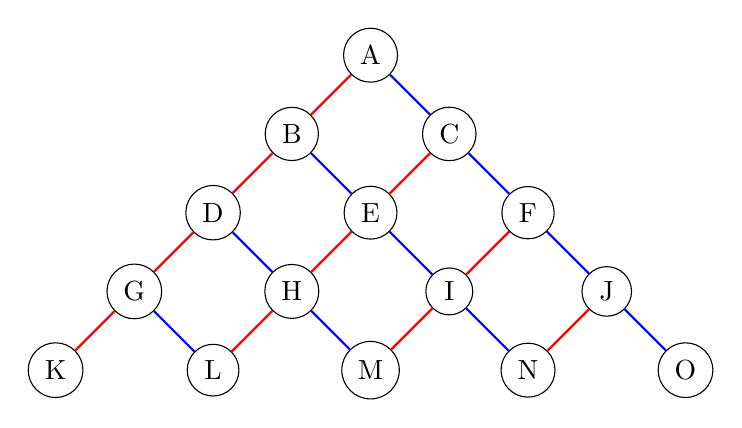
\begin{tikzpicture}

            %\draw [help lines] (0,0) grid (10,10); 

            \path   (5,10)  node (a) [circle,draw] {A}
                    (4,9) node (b) [circle,draw] {B}
                    (6,9) node (c) [circle,draw] {C}
                    (3,8) node (d) [circle,draw] {D}
                    (5,8) node (e) [circle,draw] {E}
                    (7,8) node (f) [circle,draw] {F}
                    (2,7) node (g) [circle,draw] {G}
                    (4,7) node (h) [circle,draw] {H}
                    (6,7) node (i) [circle,draw] {I}
                    (8,7) node (j) [circle,draw] {J}
                    (1,6) node (k) [circle,draw] {K}
                    (3,6) node (l) [circle,draw] {L}
                    (5,6) node (m) [circle,draw] {M}
                    (7,6) node (n) [circle,draw] {N}
                    (9,6) node (o) [circle,draw] {O};
                
            \draw[thick,red]  (node cs: name =a ) -- (node cs:name =b);
            \draw[thick,blue] (node cs: name =a ) -- (node cs:name =c);
            \draw[thick,red] (node cs: name =b ) -- (node cs:name =d);
            \draw[thick,blue] (node cs: name =b ) -- (node cs:name =e);
            \draw[thick,red] (node cs: name =d ) -- (node cs:name =g);
            \draw[thick,red] (node cs: name =c ) -- (node cs:name =e);
            \draw[thick,blue] (node cs: name =c ) -- (node cs:name =f);
            \draw[thick,red] (node cs: name =g ) -- (node cs:name =k);
            \draw[thick,blue] (node cs: name =g ) -- (node cs:name =l);
            \draw[thick,blue] (node cs: name =d ) -- (node cs:name =h);
            \draw[thick,red] (node cs: name =h ) -- (node cs:name =l);
            \draw[thick,red] (node cs: name =e ) -- (node cs:name =h);
            \draw[thick,blue] (node cs: name =h ) -- (node cs:name =m);
            \draw[thick,blue] (node cs: name =e ) -- (node cs:name =i);
            \draw[thick,red] (node cs: name =i ) -- (node cs:name =m);
            \draw[thick,blue] (node cs: name =i ) -- (node cs:name =n);
            \draw[thick,red] (node cs: name =f ) -- (node cs:name =i);
            \draw[thick,blue] (node cs: name =f ) -- (node cs:name =j);
            \draw[thick,red] (node cs: name =j ) -- (node cs:name =n);
            \draw[thick,blue] (node cs: name =j ) -- (node cs:name =o);
        \end{tikzpicture}
    \end{center}

    \begin{center}
        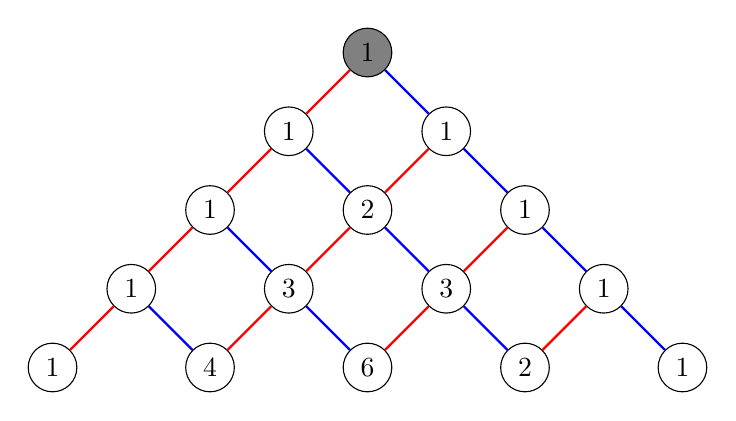
\begin{tikzpicture}

            %\draw [help lines] (0,0) grid (10,10); 

            \path   (5,10)  node (a) [circle,draw,fill = gray] {1}
                    (4,9) node (b) [circle,draw] {1}
                    (6,9) node (c) [circle,draw] {1}
                    (3,8) node (d) [circle,draw] {1}
                    (5,8) node (e) [circle,draw] {2}
                    (7,8) node (f) [circle,draw] {1}
                    (2,7) node (g) [circle,draw] {1}
                    (4,7) node (h) [circle,draw] {3}
                    (6,7) node (i) [circle,draw] {3}
                    (8,7) node (j) [circle,draw] {1}
                    (1,6) node (k) [circle,draw] {1}
                    (3,6) node (l) [circle,draw] {4}
                    (5,6) node (m) [circle,draw] {6}
                    (7,6) node (n) [circle,draw] {2}
                    (9,6) node (o) [circle,draw] {1};
                
            \draw[thick,red]  (node cs: name =a ) -- (node cs:name =b);
            \draw[thick,blue] (node cs: name =a ) -- (node cs:name =c);
            \draw[thick,red] (node cs: name =b ) -- (node cs:name =d);
            \draw[thick,blue] (node cs: name =b ) -- (node cs:name =e);
            \draw[thick,red] (node cs: name =d ) -- (node cs:name =g);
            \draw[thick,red] (node cs: name =c ) -- (node cs:name =e);
            \draw[thick,blue] (node cs: name =c ) -- (node cs:name =f);
            \draw[thick,red] (node cs: name =g ) -- (node cs:name =k);
            \draw[thick,blue] (node cs: name =g ) -- (node cs:name =l);
            \draw[thick,blue] (node cs: name =d ) -- (node cs:name =h);
            \draw[thick,red] (node cs: name =h ) -- (node cs:name =l);
            \draw[thick,red] (node cs: name =e ) -- (node cs:name =h);
            \draw[thick,blue] (node cs: name =h ) -- (node cs:name =m);
            \draw[thick,blue] (node cs: name =e ) -- (node cs:name =i);
            \draw[thick,red] (node cs: name =i ) -- (node cs:name =m);
            \draw[thick,blue] (node cs: name =i ) -- (node cs:name =n);
            \draw[thick,red] (node cs: name =f ) -- (node cs:name =i);
            \draw[thick,blue] (node cs: name =f ) -- (node cs:name =j);
            \draw[thick,red] (node cs: name =j ) -- (node cs:name =n);
            \draw[thick,blue] (node cs: name =j ) -- (node cs:name =o);
        \end{tikzpicture}
    \end{center}
   
    \begin{center}
        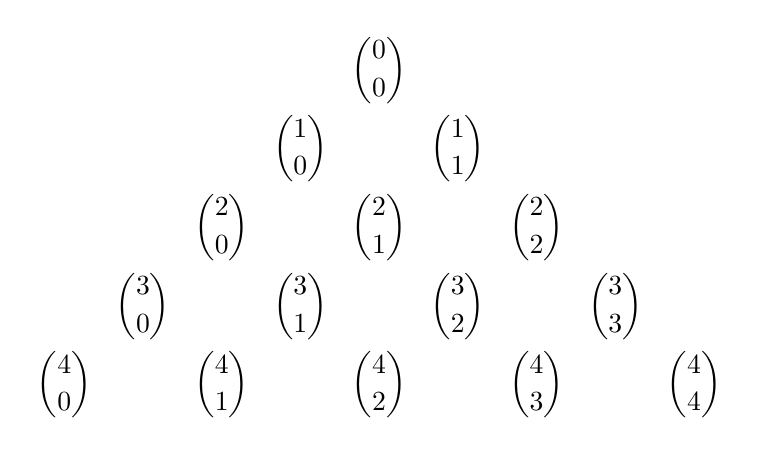
\begin{tikzpicture}

            %\draw [help lines] (0,0) grid (10,10); 

            \path   (5,10)  node (a) [] {\mbox{$\displaystyle \binom{0}{0}$ }}
                    (4,9) node (b) [] {\mbox{$\displaystyle \binom{1}{0}$ }}
                    (6,9) node (c) [] {\mbox{$\displaystyle \binom{1}{1}$ }}
                    (3,8) node (d) [] {\mbox{$\displaystyle \binom{2}{0}$ }}
                    (5,8) node (e) [] {\mbox{$\displaystyle \binom{2}{1}$ }}
                    (7,8) node (f) [] {\mbox{$\displaystyle \binom{2}{2}$ }}
                    (2,7) node (g) [] {\mbox{$\displaystyle \binom{3}{0}$ }}
                    (4,7) node (h) [] {\mbox{$\displaystyle \binom{3}{1}$ }}
                    (6,7) node (i) [] {\mbox{$\displaystyle \binom{3}{2}$ }}
                    (8,7) node (j) [] {\mbox{$\displaystyle \binom{3}{3}$ }}
                    (1,6) node (k) [] {\mbox{$\displaystyle \binom{4}{0}$ }}
                    (3,6) node (l) [] {\mbox{$\displaystyle \binom{4}{1}$ }}
                    (5,6) node (m) [] {\mbox{$\displaystyle \binom{4}{2}$ }}
                    (7,6) node (n) [] {\mbox{$\displaystyle \binom{4}{3}$ }}
                    (9,6) node (o) [] {\mbox{$\displaystyle \binom{4}{4}$ }};
                
            % \draw[thick,red]  (node cs: name =a ) -- (node cs:name =b);
            % \draw[thick,blue] (node cs: name =a ) -- (node cs:name =c);
            % \draw[thick,red] (node cs: name =b ) -- (node cs:name =d);
            % \draw[thick,blue] (node cs: name =b ) -- (node cs:name =e);
            % \draw[thick,red] (node cs: name =d ) -- (node cs:name =g);
            % \draw[thick,red] (node cs: name =c ) -- (node cs:name =e);
            % \draw[thick,blue] (node cs: name =c ) -- (node cs:name =f);
            % \draw[thick,red] (node cs: name =g ) -- (node cs:name =k);
            % \draw[thick,blue] (node cs: name =g ) -- (node cs:name =l);
            % \draw[thick,blue] (node cs: name =d ) -- (node cs:name =h);
            % \draw[thick,red] (node cs: name =h ) -- (node cs:name =l);
            % \draw[thick,red] (node cs: name =e ) -- (node cs:name =h);
            % \draw[thick,blue] (node cs: name =h ) -- (node cs:name =m);
            % \draw[thick,blue] (node cs: name =e ) -- (node cs:name =i);
            % \draw[thick,red] (node cs: name =i ) -- (node cs:name =m);
            % \draw[thick,blue] (node cs: name =i ) -- (node cs:name =n);
            % \draw[thick,red] (node cs: name =f ) -- (node cs:name =i);
            % \draw[thick,blue] (node cs: name =f ) -- (node cs:name =j);
            % \draw[thick,red] (node cs: name =j ) -- (node cs:name =n);
            % \draw[thick,blue] (node cs: name =j ) -- (node cs:name =o);
        \end{tikzpicture}

    \end{center}

    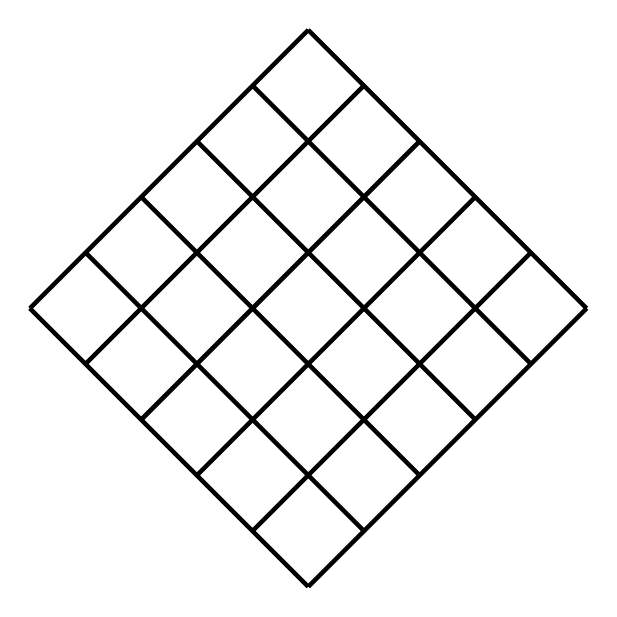
\begin{tikzpicture}
        %\draw [help lines] (0,0) grid (10,10); 
        \draw[step= 1cm,gray,ultra thick , color = black ,rotate = 45] (0,0) grid (5,5);
    \end{tikzpicture}



     
    
%Figura del TURNO 2 
    \begin{center}
        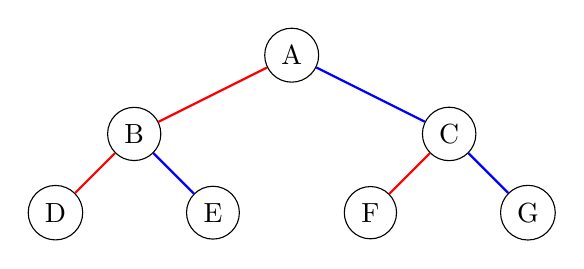
\begin{tikzpicture}

            %\draw [help lines] (0,0) grid (10,10); 

            \path   (5,10)  node (a) [circle,draw] {A}
                    (3,9) node (b) [circle,draw] {B}
                    (7,9) node (c) [circle,draw] {C}
                    (2,8) node (d) [circle,draw] {D}
                    (4,8) node (e) [circle,draw] {E}
                    (6,8) node (f) [circle,draw] {F}
                    (8,8) node (g) [circle,draw] {G};
                    
                
            \draw[thick,red]  (node cs: name =a ) -- (node cs:name =b);
            \draw[thick,blue] (node cs: name =a ) -- (node cs:name =c);
            \draw[thick,red] (node cs: name =b ) -- (node cs:name =d);
            \draw[thick,blue] (node cs: name =b ) -- (node cs:name =e);
            \draw[thick,red] (node cs: name =c ) -- (node cs:name =f);
            \draw[thick,blue] (node cs: name =c ) -- (node cs:name =g);
            
        \end{tikzpicture}
    \end{center}

    \subsection*{Turno 3}
    %TURNO 3 
    \begin{center}
        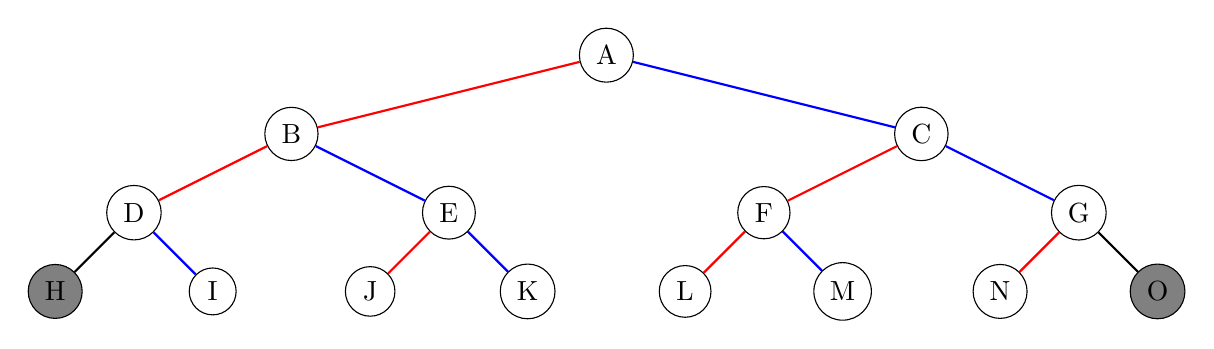
\begin{tikzpicture}

            %\draw [help lines] (0,0) grid (16,16); 

            \path   (8,10)  node (a) [circle,draw] {A}
                    (4,9) node (b) [circle,draw] {B}
                    (12,9) node (c) [circle,draw] {C}
                    (2,8) node (d) [circle,draw] {D}
                    (6,8) node (e) [circle,draw] {E}
                    (10,8) node (f) [circle,draw] {F}
                    (14,8) node (g) [circle,draw] {G}
                    (1,7) node (h) [circle,draw,fill=gray] {H}
                    (3,7) node (i) [circle,draw] {I}
                    (5,7) node (j) [circle,draw] {J}
                    (7,7) node (k) [circle,draw] {K}
                    (9,7) node (l) [circle,draw] {L}
                    (11,7) node (m) [circle,draw] {M}
                    (13,7) node (n) [circle,draw] {N}
                    (15,7) node (o) [circle,draw,fill = gray] {O};

                    
                
            \draw[thick,red]  (node cs: name =a ) -- (node cs:name =b);
            \draw[thick,blue] (node cs: name =a ) -- (node cs:name =c);
            \draw[thick,red] (node cs: name =b ) -- (node cs:name =d);
            \draw[thick,blue] (node cs: name =b ) -- (node cs:name =e);
            \draw[thick,red] (node cs: name =c ) -- (node cs:name =f);
            \draw[thick,blue] (node cs: name =c ) -- (node cs:name =g);
            \draw[thick,black] (node cs: name =d ) -- (node cs:name =h);
            \draw[thick,red] (node cs: name =e ) -- (node cs:name =j);
            \draw[thick,red] (node cs: name =f ) -- (node cs:name =l);
            \draw[thick,red] (node cs: name =g) -- (node cs:name =n);
            \draw[thick,blue] (node cs: name =d ) -- (node cs:name =i);
            \draw[thick,blue] (node cs: name =e ) -- (node cs:name =k);
            \draw[thick,blue] (node cs: name =f) -- (node cs:name =m);
            \draw[thick,black] (node cs: name =g ) -- (node cs:name =o);
            
        \end{tikzpicture}
    \end{center}



    \subsubsection*{Turno 3.1}
    %TURNO 3 
    \begin{center}
        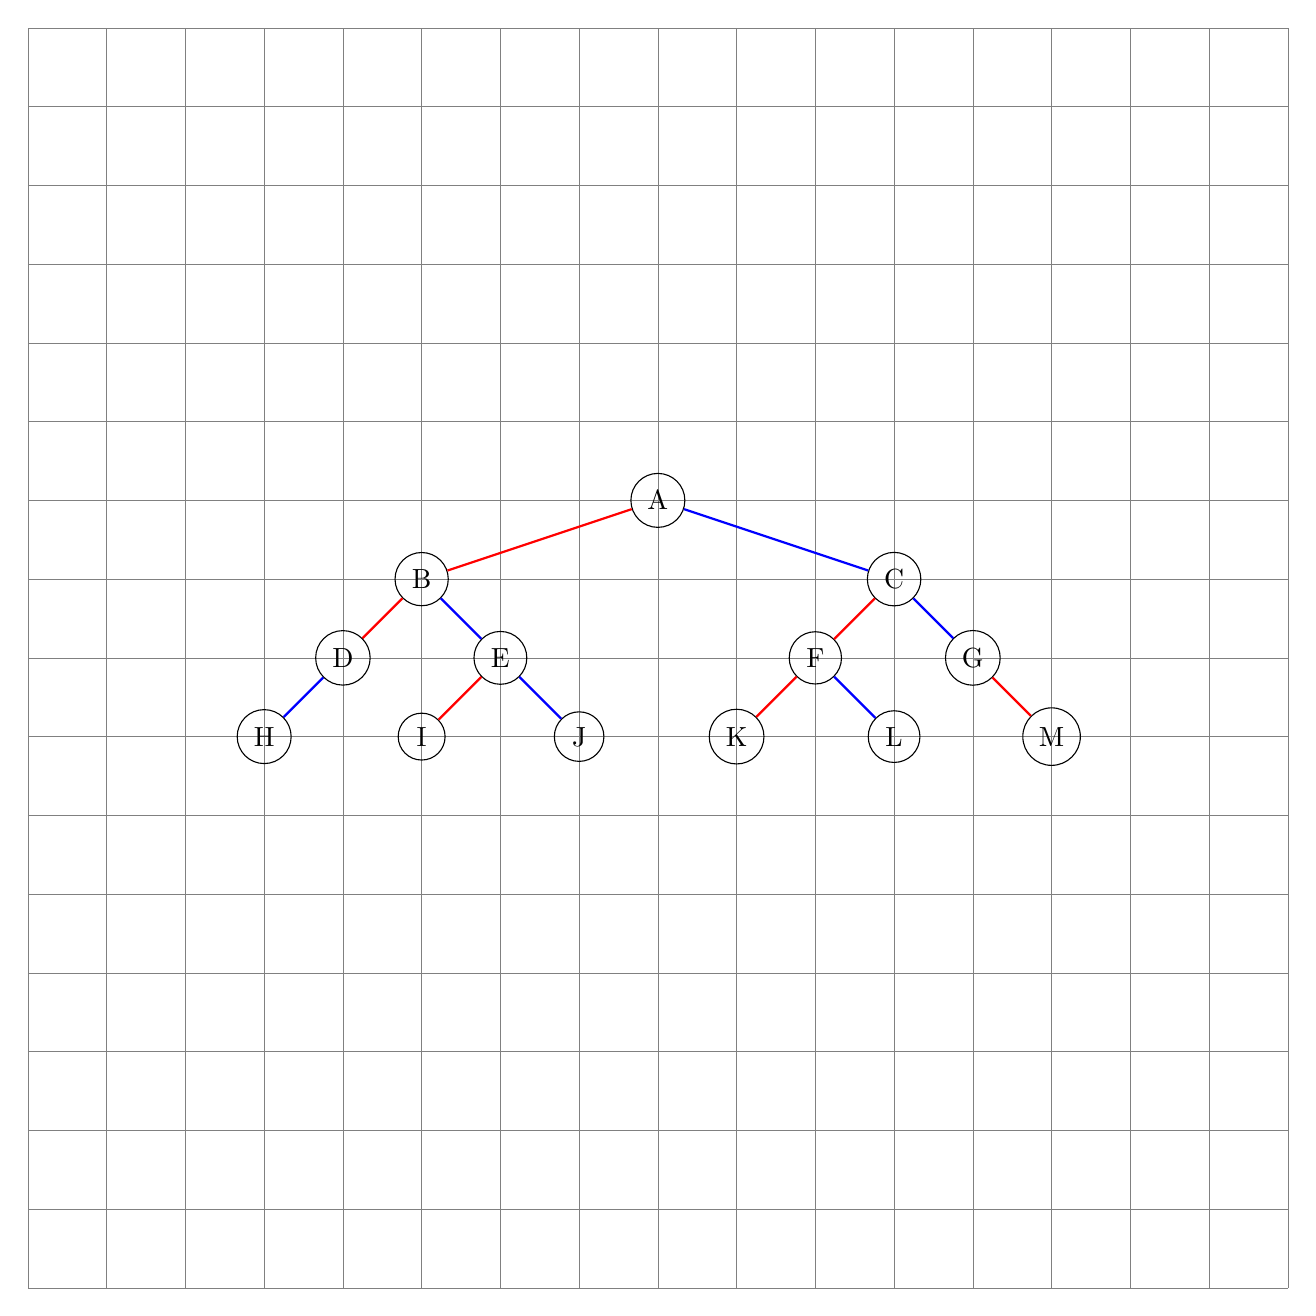
\begin{tikzpicture}

            \draw [help lines] (0,0) grid (16,16); 

            \path   (8,10)  node (a) [circle,draw] {A}
                    (5,9) node (b) [circle,draw] {B}
                    (11,9) node (c) [circle,draw] {C}
                    (4,8) node (d) [circle,draw] {D}
                    (6,8) node (e) [circle,draw] {E}
                    (10,8) node (f) [circle,draw] {F}
                    (12,8) node (g) [circle,draw] {G}
                    (3,7) node (h) [circle,draw] {H}
                    (5,7) node (i) [circle,draw] {I}
                    (7,7) node (j) [circle,draw] {J}
                    (9,7) node (k) [circle,draw] {K}
                    (11,7) node (l) [circle,draw] {L}
                    (13,7) node (m) [circle,draw] {M};
                    %(13,7) node (n) [circle,draw] {N}
                    %(15,7) node (o) [circle,draw] {O};

                    
                
            \draw[thick,red]  (node cs: name =a ) -- (node cs:name =b);
            \draw[thick,blue] (node cs: name =a ) -- (node cs:name =c);
            \draw[thick,red] (node cs: name =b ) -- (node cs:name =d);
            \draw[thick,blue] (node cs: name =b ) -- (node cs:name =e);
            \draw[thick,red] (node cs: name =c ) -- (node cs:name =f);
            \draw[thick,blue] (node cs: name =c ) -- (node cs:name =g);
            \draw[thick,blue] (node cs: name =d ) -- (node cs:name =h);
            \draw[thick,red] (node cs: name =e ) -- (node cs:name =i);
            \draw[thick,blue] (node cs: name =e ) -- (node cs:name =j);
            \draw[thick,red] (node cs: name =f) -- (node cs:name =k);
            \draw[thick,blue] (node cs: name =f ) -- (node cs:name =l);
            \draw[thick,red] (node cs: name =g ) -- (node cs:name =m);
            %\draw[thick,blue] (node cs: name =f) -- (node cs:name =m);
            %\draw[thick,black] (node cs: name =g ) -- (node cs:name =o);
            
        \end{tikzpicture}
    \end{center}

\end{document}